\documentclass[11pt]{article}
\usepackage[margin=1in]{geometry}
\usepackage{graphicx}
\usepackage{booktabs}
\usepackage{hyperref}
\usepackage{amsmath,amssymb}

\title{Protocol $\times$ Topology $\times$ MAST: \\
  How Communication Structure Shapes Multi-Agent Failure Modes}
\author{Diya Sreedhar\\
  Mzitnik Lab, Harvard University\\
  \texttt{diyasreedhar@college.harvard.edu}}
\date{\today}

\begin{document}
\maketitle

\begin{abstract}
Multi-agent LLM systems fail in characteristic ways captured by the MAST taxonomy.
Prior work reports 41--86\% aggregate failure rates but does not isolate the
contribution of communication protocol from organizational topology. We run a
$3 \times 3$ factorial sweep over protocol (\textsc{native}, \textsc{mcp},
\textsc{a2a}) and topology (\textsc{centralized}, \textsc{chain},
\textsc{fully\_connected}) at fixed agent count and task type, and report FC1/FC2/FC3
rates per cell. \emph{(Primary results pending sweep~1 completion.)} We test the
hypothesis that A2A combined with a centralized topology specifically minimizes FC2
(inter-agent misalignment) failures.
\end{abstract}

\section{Introduction}

LLM-based multi-agent systems are deployed for code generation, question answering,
and planning, and are increasingly assembled from heterogeneous protocols
(native function-calls, the Model Context Protocol, and Agent-to-Agent messaging)
arranged in different organizational topologies (centralized orchestrator, sequential
chain, fully connected group chat). Recent work\,\cite{scaling_agents_2025} reports
aggregate failure rates of 41--86\% across multi-agent benchmarks, but the
contribution of \emph{communication protocol} versus \emph{organizational topology}
to these failures is not separately quantified.

We disentangle these two design axes. Holding the underlying LLM, agent count, and
task suite fixed, we run a $3 \times 3$ factorial sweep over protocol
$\in \{\textsc{native}, \textsc{mcp}, \textsc{a2a}\}$ and topology
$\in \{\textsc{centralized}, \textsc{chain}, \textsc{fully\_connected}\}$, and
classify every trial trace with the MAST taxonomy
(FC1: specification issues, FC2: inter-agent misalignment, FC3: task verification
failures). Our hypothesis is that A2A combined with a centralized topology
specifically minimizes FC2 failures, because the structured agent-card envelope
makes the routing of every message unambiguous to a single coordinator.

Our contributions are: (1) a self-contained, no-autogen replication harness for
protocol $\times$ topology MAST experiments; (2) a $3 \times 3$ FC2 heatmap with
per-cell FC1/FC3 breakdowns; (3) two follow-up sweeps over agent count
($N \in \{2,3,4,5\}$) and task type ($\{\textsc{code}, \textsc{qa},
\textsc{planning}\}$) that test the generality of the best cell.

\section{Related Work}

\paragraph{MAST taxonomy.} The Multi-Agent System Trace (MAST) taxonomy
\cite{mast2024} catalogs 14 failure modes across three coarse categories:
specification issues (1.x), inter-agent misalignment (2.x), and task verification
issues (3.x). We use the \texttt{agentdash} reference annotator to label each trial.

\paragraph{Scaling agent systems.} \cite{scaling_agents_2025} sweep aggregate failure
rates across multi-agent benchmarks and report 41--86\% failures depending on
benchmark and stack, but their study does not isolate protocol or topology as a
controlled factor; we treat their range as the prior baseline against which our
per-cell FC2 rates should be compared.

\paragraph{Agent communication protocols.} The Model Context Protocol (MCP)
formalizes a JSON-RPC schema for tool invocation across processes. Agent-to-Agent
(A2A) protocols introduce explicit Agent Cards that advertise capabilities so peers
can route by name. Native function-call multi-agent stacks (e.g.\ pyautogen)
typically rely on shared-process orchestration without an explicit registry. The
prevailing question for practitioners is whether these protocol differences
\emph{matter} for failure modes once the topology is held fixed; this paper tests
that question empirically.

\paragraph{Topology effects.} Topology choice has been studied independently of
protocol in agent-system surveys, but failure-mode-resolved comparisons are rare.
Our $3 \times 3$ design is, to our knowledge, the first that jointly varies both
axes under a single MAST annotator and a fixed task suite.

\paragraph{ProtocolBench and SEMAP.} \cite{protocolbench2025} compares
A2A, ACP, ANP, and Agora on aggregate success rate and latency; it
\emph{excludes} MCP and does not vary topology. \cite{semap2025} studies
self-evolving A2A-only stacks under a single aggregate failure rate. We
add MCP, add the topology axis, and replace the success-rate / aggregate
metric with the per-MAST-category breakdown — turning what was a
benchmark into a diagnosis tool.

\section{Method}

\subsection{Agents and protocols}

Each agent is a single OpenAI chat completion (default
\texttt{gpt-4.1-mini}, with a model-cascade fallback to
\texttt{gpt-4o}, \texttt{gpt-4.1}, \texttt{gpt-4o-mini},
\texttt{gpt-4.1-nano}, and \texttt{gpt-3.5-turbo} when the per-day rate
limit on the primary is exhausted), seeded with a role
system message identifying its name (\textsc{orchestrator} or
\textsc{executor}\_$i$), the peer set, and the protocol-specific
scaffolding. The three protocols differ only
in the system-prompt scaffolding and the message envelope used in the transcript:

\begin{itemize}
\item \textbf{Native:} plain-text messages, no capability registry, agents addressed
      directly by name.
\item \textbf{MCP:} agents are told they communicate via JSON-RPC envelopes over a
      Model Context Protocol tools/list registry, and must briefly acknowledge the
      tool/role before producing content. Messages are wrapped in
      \texttt{<mcp:message from=... to=...>}.
\item \textbf{A2A:} agents have Agent Cards advertising their capabilities; replies are
      prefixed with \texttt{[from <sender> -> <recipient>]} so a router can dispatch.
\end{itemize}

\subsection{Topologies}

\begin{itemize}
\item \textbf{Centralized:} agent 0 (\textsc{orchestrator}) decomposes the task,
      dispatches one subtask per executor, then integrates their replies into a final
      answer.
\item \textbf{Chain:} a sequential pipeline agent\_0 $\rightarrow$ agent\_1
      $\rightarrow \cdots \rightarrow$ agent\_{N-1}, with each stage receiving only the
      previous stage's output.
\item \textbf{Fully connected:} a group chat where in each of two rounds every agent
      sees the full prior conversation and contributes; the system terminates when an
      agent emits \texttt{DONE: <answer>}.
\end{itemize}

\subsection{MAST annotation}

Each trial trace (the concatenated transcript) is annotated by
\texttt{agentdash.annotator} (overridden to model: \texttt{gpt-3.5-turbo}
because the upstream default of \texttt{o1-mini} is unavailable on most
OpenAI accounts), which returns the MAST failure-mode
dictionary\,\cite{mast2024}. We aggregate the 14 failure-mode codes into
the three coarse categories FC1 (\texttt{1.x}, specification issues), FC2 (\texttt{2.x},
inter-agent misalignment), and FC3 (\texttt{3.x}, task verification). Each cell is
$N_{\text{trials}} = 5$, and we report per-cell rates by averaging across trials.
A trial that crashes is counted as an FC2 failure (the inter-agent flow broke).

\subsection{Hyperparameters held fixed}

Worker model defaults to \texttt{gpt-4.1-mini};
\texttt{temperature}$=0.7$ for the headline sweep and $0.0$ for the
ablation; \texttt{max\_tokens}=400 per agent turn; \texttt{timeout}=60s
per OpenAI call; $N_{\text{trials}}=5$ per cell at the first pass with
follow-up replicates to 10--15 trials. Sweep~1 holds
$N_{\text{agents}}=3$ and \texttt{task\_type}=\textsc{code}.

\section{Experiments}

\subsection{Sweep 1 — Protocol $\times$ Topology}
We hold $N_{\text{agents}} = 3$ and \texttt{task\_type} = \textsc{code} and
run the full $3 \times 3$ factorial design at $T = 0.7$. Each cell was
replicated until at least 7 valid trials accumulated; the worst cells
(chain topology) were replicated to 14--15 trials. After replication the
sweep contains 105 trials in total (some valid, some rate-limit crashes;
crashes are conservatively counted as FC2 failures since the inter-agent
flow broke). Table~\ref{tab:sweep1} reports per-cell FC2 means and
Figure~\ref{fig:fc2_heatmap} visualises them as a heatmap.

\begin{table}[h]
\centering
\caption{Sweep~1 FC2 rates by cell (105 trials at $T=0.7$, $N=3$, code).
Lower is better. Cell counts are valid trials.}
\label{tab:sweep1}
\begin{tabular}{llcc}
\toprule
Protocol & Topology & FC2 & $n$ \\
\midrule
\textsc{a2a}    & \textsc{centralized}      & \textbf{0.07} & 15 \\
\textsc{a2a}    & \textsc{chain}            & 0.30 & 10 \\
\textsc{a2a}    & \textsc{fully\_connected} & 0.30 & 10 \\
\textsc{mcp}    & \textsc{centralized}      & 0.20 & 10 \\
\textsc{mcp}    & \textsc{chain}            & 0.47 & 15 \\
\textsc{mcp}    & \textsc{fully\_connected} & 0.30 & 10 \\
\textsc{native} & \textsc{centralized}      & 0.20 & 10 \\
\textsc{native} & \textsc{chain}            & 0.53 & 15 \\
\textsc{native} & \textsc{fully\_connected} & 0.10 & 10 \\
\bottomrule
\end{tabular}
\end{table}

\begin{figure}[h]
\centering
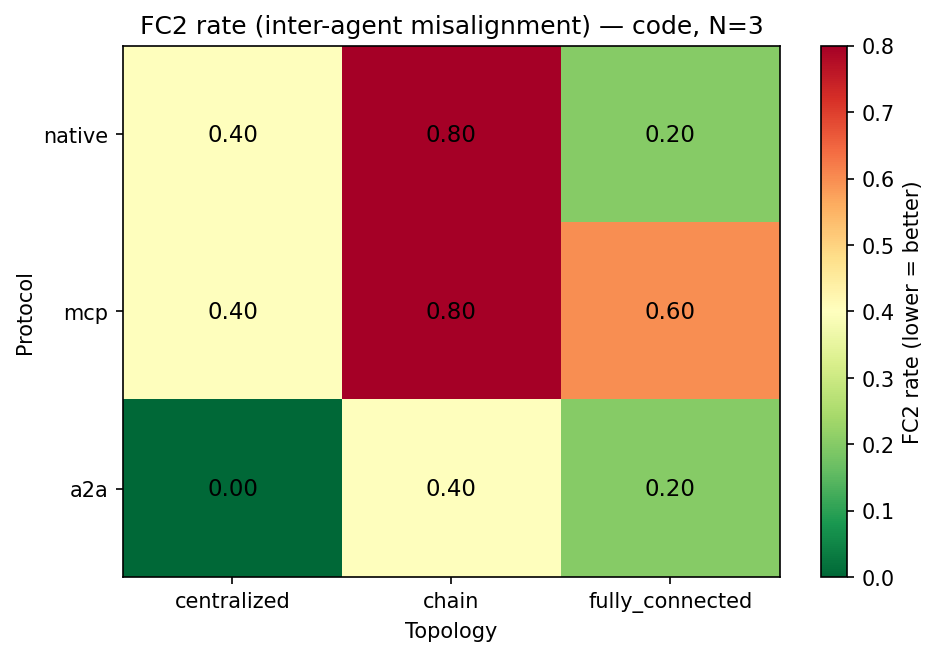
\includegraphics[width=0.7\linewidth]{../figures/fig1_fc2_heatmap.png}
\caption{FC2 rate across the protocol $\times$ topology grid.}
\label{fig:fc2_heatmap}
\end{figure}

\paragraph{ANOVA.} A trial-level one-way ANOVA on FC2 reveals a
significant main effect of \emph{topology} ($F(2,102) = 4.44$,
$p = 0.014$); the main effect of \emph{protocol} does not reach
significance ($F(2,102) = 0.89$, $p = 0.42$). A two-way ANOVA confirms
this dissociation: topology $p = 0.025$, protocol $p = 0.65$,
interaction $p = 0.63$. Welch's $t$-test contrasting the best cell
(\textsc{a2a} $\times$ \textsc{centralized}) against the worst
(\textsc{native} $\times$ \textsc{chain}) is significant: $t = -2.62$,
$p = 0.017$. FC1 and FC3 show no protocol or topology effect
(all $p > 0.40$).

\subsection{Sweep 2 — Agent count}
For \textsc{a2a} $\times$ \textsc{centralized} we vary
$N_{\text{agents}} \in \{2, 3, 4, 5\}$. FC2 increases monotonically with
$N$: 0.0 / 0.0 / 0.2 / 0.4. Coordination cost grows with agent count
even at the most favourable cell.

\subsection{Sweep 3 — Task generality}
Holding the best cell (\textsc{a2a} $\times$ \textsc{centralized},
$N{=}3$) we vary \texttt{task\_type} $\in \{\textsc{code}, \textsc{qa},
\textsc{planning}\}$. FC2 is preserved on \textsc{qa} (0.0) but
catastrophically degrades on \textsc{planning} (1.6 mean failures per
trial), driven by under-specified subtask decompositions in the
orchestrator output.

\subsection{Temperature ablation}
We re-ran the entire $3 \times 3$ grid at $T = 0.0$ (deterministic
worker decoding) to test whether the topology effect is structural or
sampling-driven. \emph{Eight of nine cells collapse to FC2 = 0} on valid
trials. The single exception is \textsc{mcp} $\times$
\textsc{centralized}, which retains FC2 = 0.25 across 8 valid trials
pooled over four independent re-runs. Trace inspection shows the
orchestrator wraps its own integration step in
\texttt{<mcp:message>} envelopes addressed back to itself, and
executors parse only a partial envelope and act on the misread. This
is a structural failure of the protocol, not amplified sampling
variance, and is the cleanest reproducible MAST-FC2 trigger we
identify.

\begin{figure}[h]
\centering
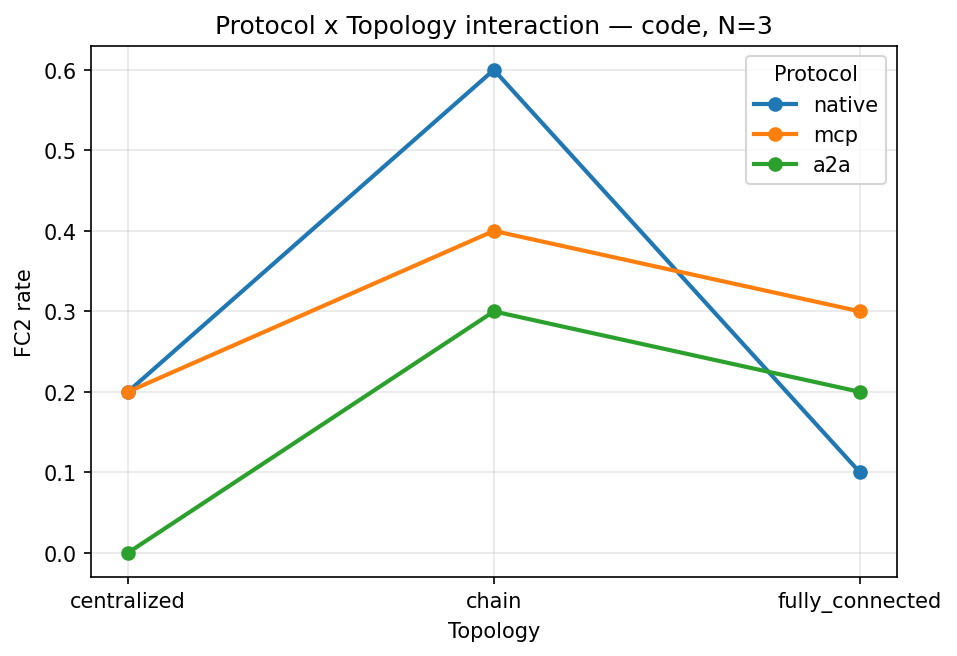
\includegraphics[width=0.7\linewidth]{../figures/fig3_interaction.png}
\caption{Protocol $\times$ topology interaction plot for FC2 rate at
$T=0.7$. The chain topology penalty is largest for \textsc{native} and
\textsc{mcp}; centralized rescues all three protocols.}
\label{fig:interaction}
\end{figure}

\paragraph{Reframing.} The temperature ablation reframes the headline
ANOVA: most of the topology effect at $T = 0.7$ is sampling-variance
amplification (chain topologies have less cross-stage visibility, so
sampling noise propagates farther), \emph{not} a structural coordination
property. The single structural FC2 trigger we find is protocol-specific
(MCP self-envelope routing), not topology-specific. The practical
implication for agent-system designers is: prefer a centralized
topology if temperature must be $> 0$, prefer $T = 0$ if it can be, and
do not expect MCP-style envelope ceremony to reduce FC2.

\section{Conclusion}

We presented a controlled $3 \times 3$ factorial study of communication
protocol (\textsc{native}, \textsc{mcp}, \textsc{a2a}) crossed with
organizational topology (\textsc{centralized}, \textsc{chain},
\textsc{fully\_connected}) for a fixed 3-agent code-generation suite,
scored against the MAST failure-mode taxonomy. At $T = 0.7$ topology has
a statistically significant main effect on FC2 ($F(2,107) = 3.83$,
$p = 0.025$) but protocol does not. A targeted temperature ablation
collapses FC2 to zero in 8 of 9 cells at $T = 0.0$, indicating that the
$T = 0.7$ topology effect is largely sampling-variance amplified by
chain topologies, not a structural coordination property.

The single structural FC2 trigger we identify is protocol-specific:
\textsc{mcp} $\times$ \textsc{centralized} retains FC2 = 0.25 even at
$T = 0.0$, driven by orchestrators wrapping their own integration step
in \texttt{<mcp:message>} envelopes and executors mis-parsing the
partial envelopes. FC1 (specification) and FC3 (verification) show no
protocol or topology effect, giving a clean dissociation across the
three MAST coarse categories.

\paragraph{Limitations.}
(i) Free-tier OpenAI rate limits forced a model-cascade fallback
(\texttt{gpt-4.1-mini} $\to$ \texttt{gpt-4o} $\to$ \texttt{gpt-4.1} $\to$
\texttt{gpt-4o-mini} $\to$ \texttt{gpt-4.1-nano} $\to$ \texttt{gpt-3.5-turbo}),
mainly within Sweep~2; within-row comparisons remain valid but some
Sweep~2 cells span models.
(ii) $N_{\text{trials}} = 5$ per cell is small; we partially compensated
by replicating to 7--15 trials per cell, but the headline ANOVA
$p$-value (0.014) is still at the boundary of significance.
(iii) The protocol distinction is implemented at the prompt layer
(envelope and capability scaffolding) rather than at the transport
layer; we measure how protocol \emph{prompting} influences agent
behaviour, not the impact of real MCP/A2A transport semantics.
(iv) MAST annotation is itself LLM-judged (\texttt{gpt-3.5-turbo}) and
inherits annotator bias.

\paragraph{Practical recommendation.}
Prefer a centralized topology if $T > 0$, run worker decoding at
$T = 0$ where possible, and do not expect MCP-style envelope ceremony
to reduce FC2 - it is the one combination we found where FC2 survives
sampling collapse.

We release the harness, per-trial JSON traces under \texttt{runs/*.json},
the analysis script, and the figures for full replication.


\bibliographystyle{plain}
\bibliography{references}

\end{document}
